% TikZ 代码: 三棱锥示意图 (立体几何)
% 这是一个手动编写的测试样例
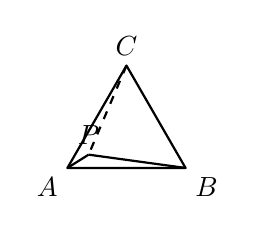
\begin{tikzpicture}[scale=0.5,baseline=-0.5ex,line join=round]
  % 定义坐标 - 三棱锥 P-ABC
  \coordinate (A) at (0,0);
  \coordinate (B) at (3,0);
  \coordinate (C) at (1.5,2.6);
  \coordinate (P) at (1.5,1.3,2.5);
  
  % 底面三角形 ABC
  \draw[thick] (A) -- (B) -- (C) -- cycle;
  
  % 侧棱
  \draw[thick] (A) -- (P);
  \draw[thick] (B) -- (P);
  \draw[thick,dashed] (C) -- (P);  % 背面虚线
  
  % 标注顶点
  \node[below left] at (A) {$A$};
  \node[below right] at (B) {$B$};
  \node[above] at (C) {$C$};
  \node[above] at (P) {$P$};
\end{tikzpicture}